%---------------------------------------------------------------------
\section{Resultados das simula��es}

Nas simula��es, procuramos avaliar o comportamento do sistema para as seguintes condi��es:
%
\begin{enumerate*}[label=(\roman*)]
\item condi��es iniciais $\theta(0)$ e $y(0)$;
\item Par�metros da planta e do modelo;
\item ganho de adapta��o $\Gamma$.
\end{enumerate*}

Apresentaremos os resultados obtidos atrav�s de simula��es no ambiente \HI{\texttt{Matlab/Simulink}} e os discutiremos na pr�xima se��o.

\subsection{Simula��o \#1}

Inicialmente, desejamos verificar o comportamento do sistema para varia��es nas
condi��es iniciais.

\bigskip

\textbf{\underline{Simula��o 1.1}: $\theta(0)$}
%
\begin{align*}
  y &= \frac{5}{s^2+2s+1}u\,,  &  \theta(0) &= \HI{0} \, \textrm{e} \, \HI{1}\,,
  & y(0) &= 0 \,, & \Gamma &= 1 \, \textbf{I}_3\,, \\ y_r &= \textrm{sin}(t) +
  \textrm{sin}(3t) \, .
\end{align*}

\begin{figure}[H]
  \centering
  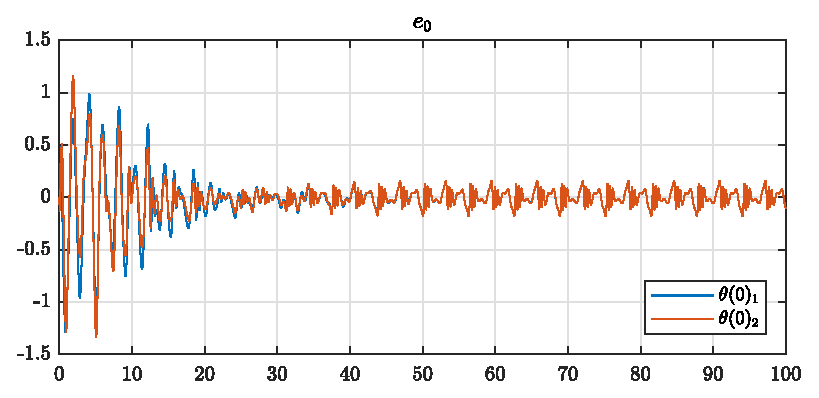
\includegraphics[width=12cm]{figs/e0/sim0_theta0.eps} 
\end{figure}

\begin{figure}[H]
  \centering
  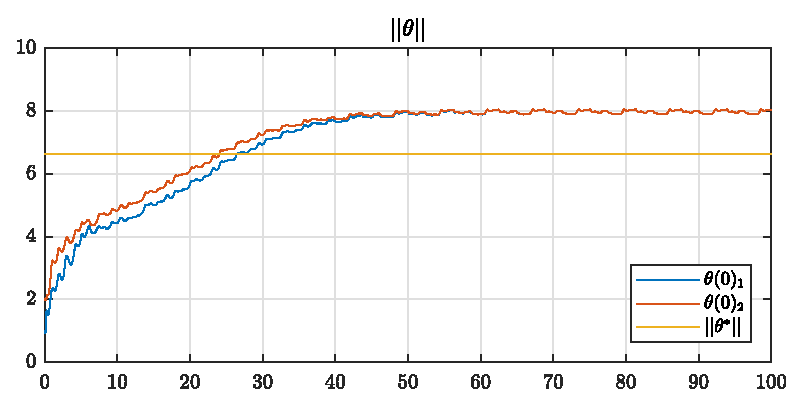
\includegraphics[width=12cm]{figs/modtheta/sim0_theta0.eps} 
\end{figure}

\begin{figure}[H]
  \centering
  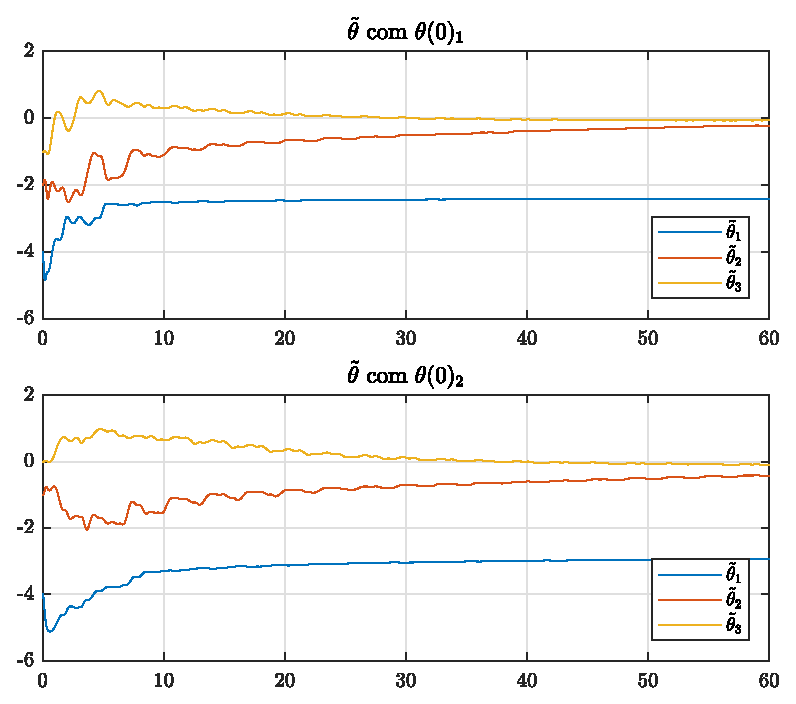
\includegraphics[width=12cm]{figs/tiltheta/sim0_theta0.eps} 
\end{figure}

\begin{figure}[H]
  \centering
  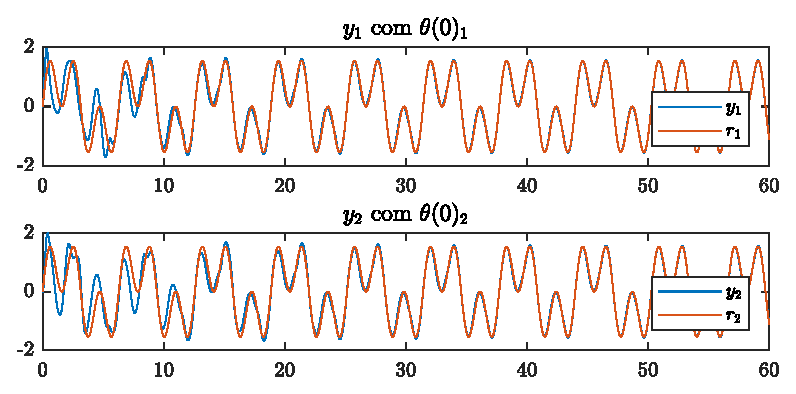
\includegraphics[width=12cm]{figs/y/sim0_theta0.eps} 
\end{figure}

\textbf{\underline{Simula��o 1.2}: $y(0)$}
%
\begin{align*}
  y &= \frac{5}{s^2+2s+1}u\,,  &  \theta(0) &= 0 \,,
  & y(0) &=  \HI{0} \, \textrm{e} \, \HI{5} \,, & \Gamma &= 1 \,
  \textbf{I}_3\,, \\ y_r &= \textrm{sin}(t) + \textrm{sin}(3t) \, .
\end{align*}

\begin{figure}[H]
  \centering
  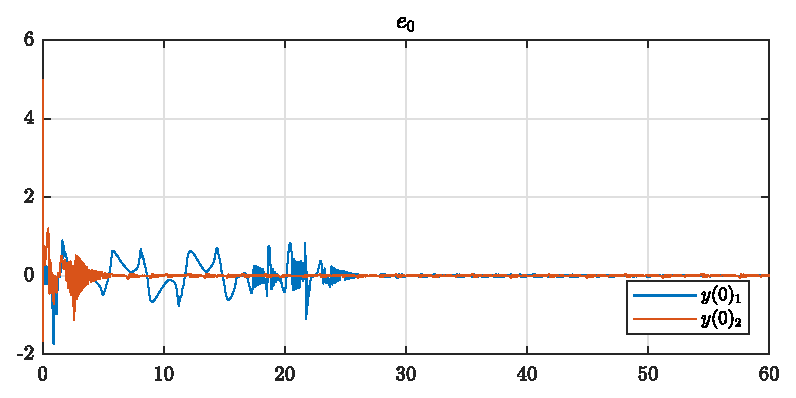
\includegraphics[width=12cm]{figs/e0/sim0_y.eps} 
\end{figure}

\begin{figure}[H]
  \centering
  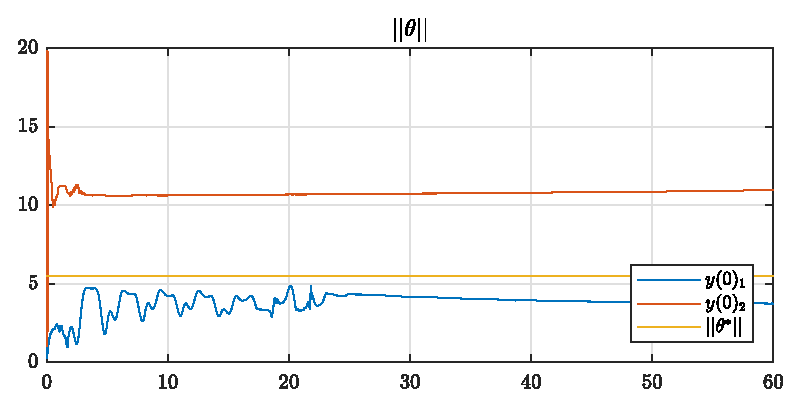
\includegraphics[width=12cm]{figs/modtheta/sim0_y.eps} 
\end{figure}

\begin{figure}[H]
  \centering
  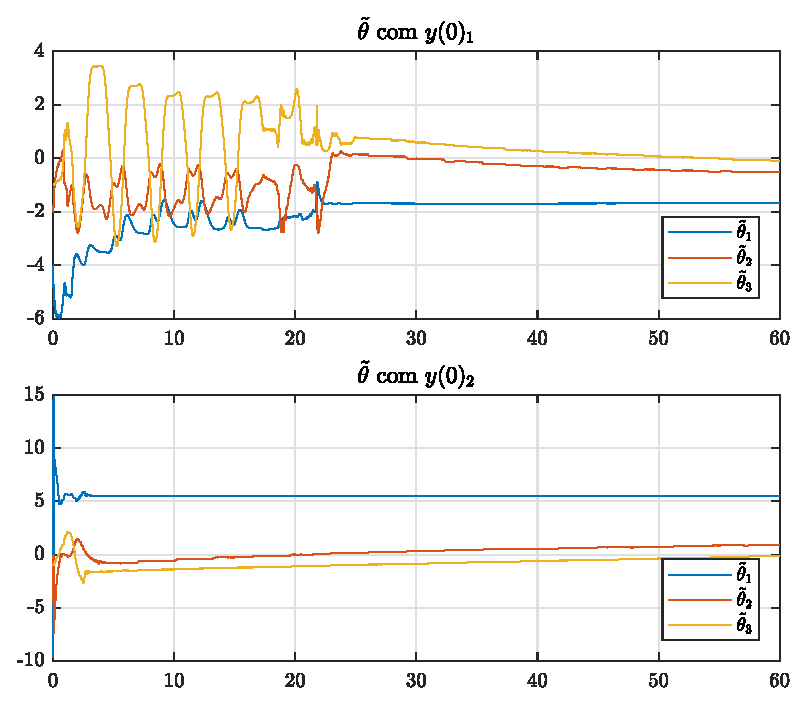
\includegraphics[width=12cm]{figs/tiltheta/sim0_y.eps} 
\end{figure}

\begin{figure}[H]
  \centering
  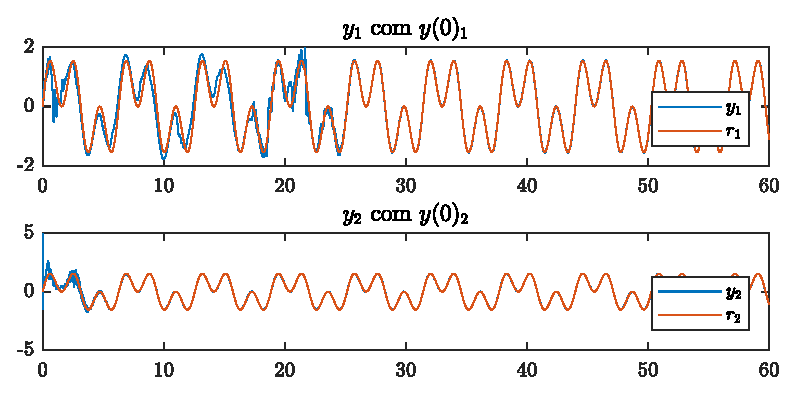
\includegraphics[width=12cm]{figs/y/sim0_y.eps} 
\end{figure}

\subsection{Simula��o \#2}

Verificamos o comportamento do sistema para varia��es no par�metro de adapta��o
$\Gamma$.

\bigskip

\begin{align*}
  y &= \frac{5}{s^2+2s+1}u\,,  &  \theta(0) &= 0 \,,
  & y(0) &=  0 \,, & \Gamma &= \HI{1} \, \textrm{e} \, \HI{5} \,
  \textbf{I}_3\,, \\ y_r &= \textrm{sin}(t) + \textrm{sin}(3t) \, .
\end{align*}

\begin{figure}[H]
  \centering
  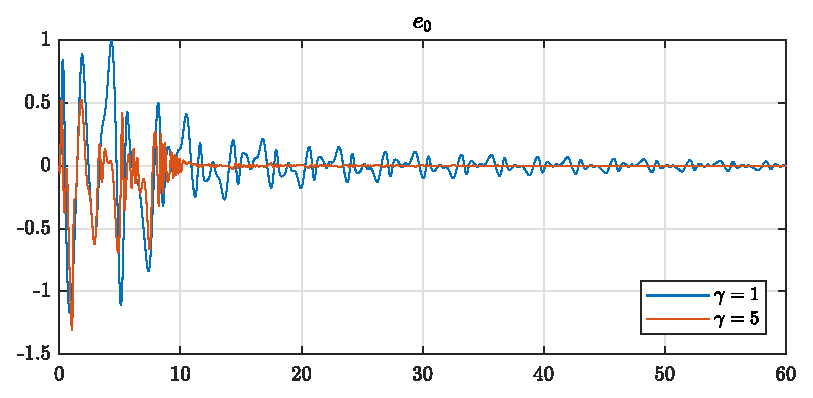
\includegraphics[width=12cm]{figs/e0/sim0_gamma1gamma5.eps} 
\end{figure}

\begin{figure}[H]
  \centering
  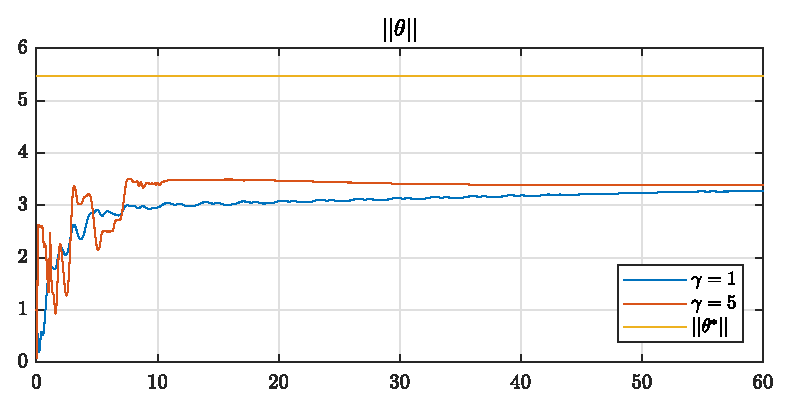
\includegraphics[width=12cm]{figs/modtheta/sim0_gamma1gamma5.eps} 
\end{figure}

\begin{figure}[H]
  \centering
  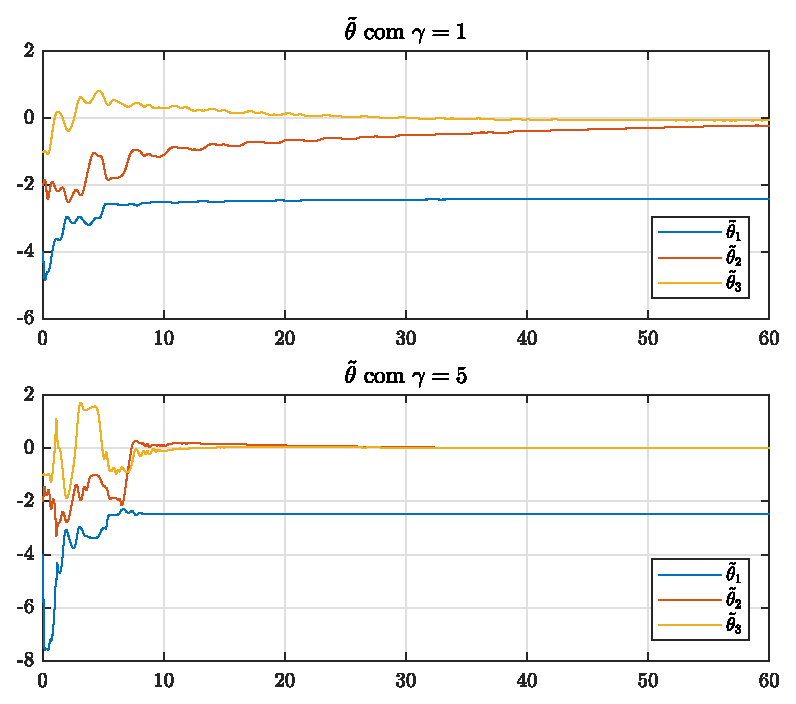
\includegraphics[width=12cm]{figs/tiltheta/sim0_gamma1gamma5.eps} 
\end{figure}

\begin{figure}[H]
  \centering
  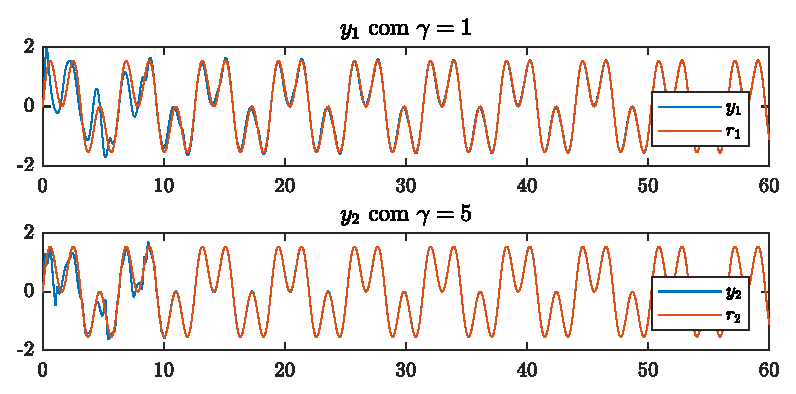
\includegraphics[width=12cm]{figs/y/sim0_gamma1gamma5.eps} 
\end{figure}

\subsection{Simula��o \#3}

Verificamos o comportamento do sistema para varia��es na planta e modelo.

\bigskip

\textbf{\underline{Simula��o 3.1}: planta}
%
\begin{align*}
  y &= \frac{5}{s^2+2s+1}u\, \textrm{e} \, \frac{5}{s^2-2s+1}u,  &  \theta(0) &=
  0 \,, & y(0) &=  0 \,, & \Gamma &= 1 \,
  \textbf{I}_3\,, \\ y_r &= \textrm{sin}(t) + \textrm{sin}(3t) \, .
\end{align*}

\begin{figure}[H] 
  \centering
  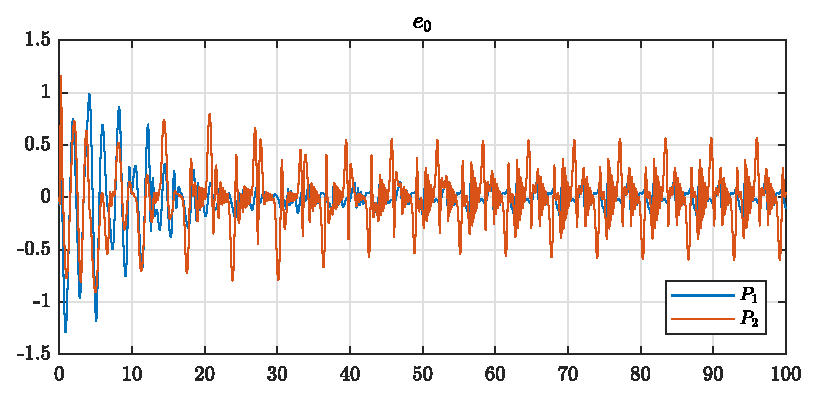
\includegraphics[width=12cm]{figs/e0/sim0_P1P2.eps} 
\end{figure}

\begin{figure}[H]
  \centering
  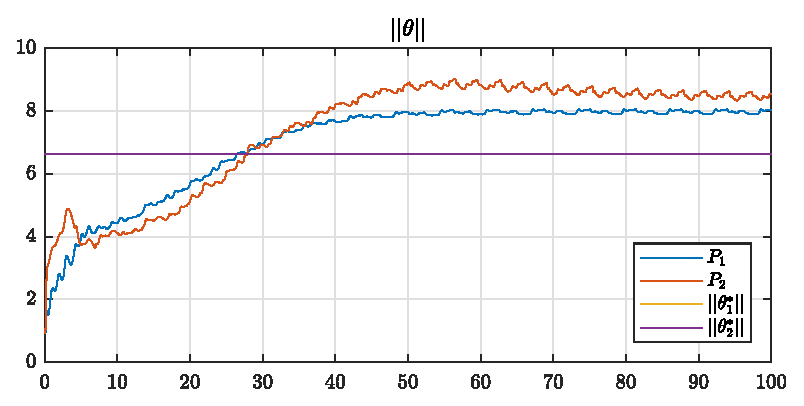
\includegraphics[width=12cm]{figs/modtheta/sim0_P1P2.eps} 
\end{figure}

\begin{figure}[H]
  \centering
  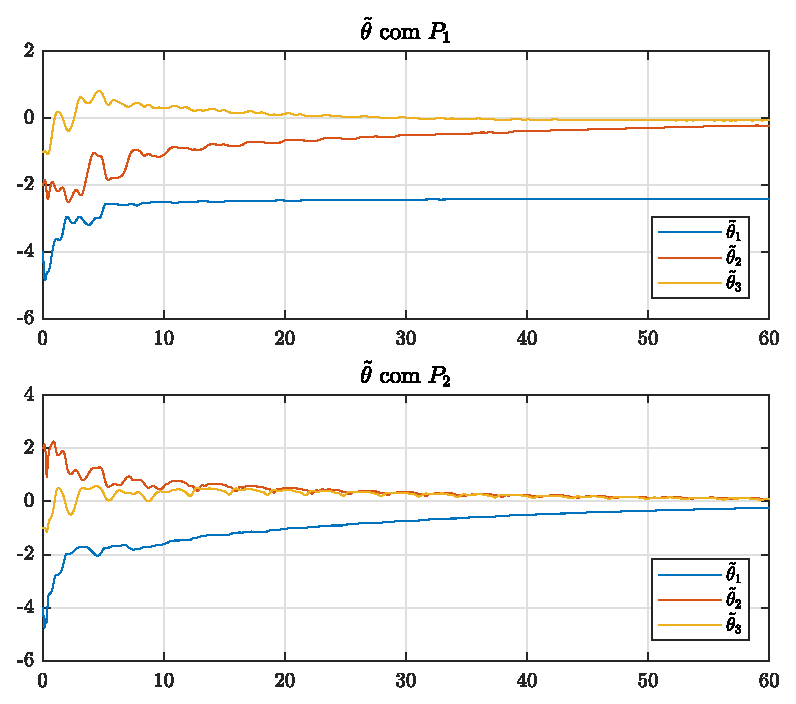
\includegraphics[width=12cm]{figs/tiltheta/sim0_P1P2.eps} 
\end{figure}

\begin{figure}[H]
  \centering
  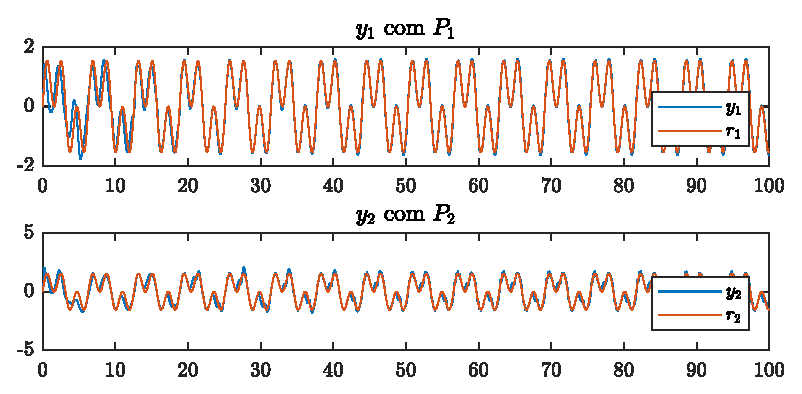
\includegraphics[width=12cm]{figs/y/sim0_P1P2.eps} 
\end{figure}

\textbf{\underline{Simula��o 3.2}: modelo}
%
\begin{align*}
  y &= \frac{5}{s^2+2s+1}u\, &  \theta(0) &=
  0 \,, & y(0) &=  0 \,, & \Gamma &= 1 \,
  \textbf{I}_3\,, \\ y_r &= \textrm{sin}(t) + \textrm{sin}(3t) \, \textrm{e} \,
  \textrm{sin}(t) + \textrm{2sin}(5t) .
\end{align*}
 
\begin{figure}[H]
  \centering
  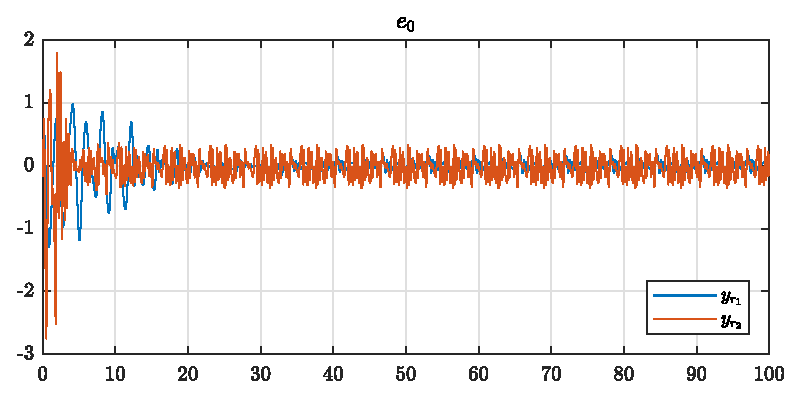
\includegraphics[width=12cm]{figs/e0/sim0_yr1yr2.eps} 
\end{figure}

\begin{figure}[H]
  \centering
  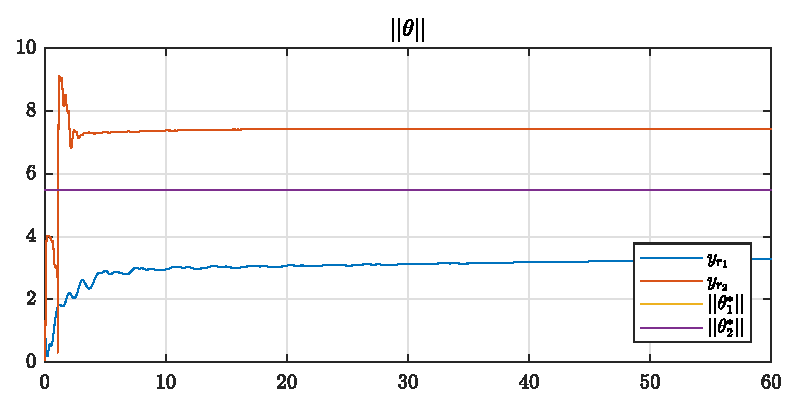
\includegraphics[width=12cm]{figs/modtheta/sim0_yr1yr2.eps} 
\end{figure}

\begin{figure}[H]
  \centering
  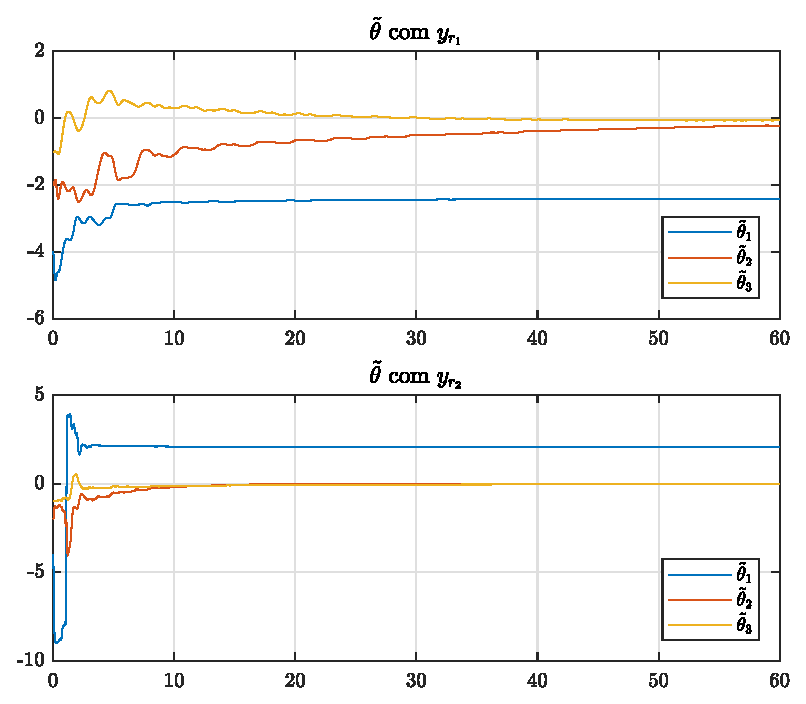
\includegraphics[width=12cm]{figs/tiltheta/sim0_yr1yr2.eps} 
\end{figure}

\begin{figure}[H]
  \centering
  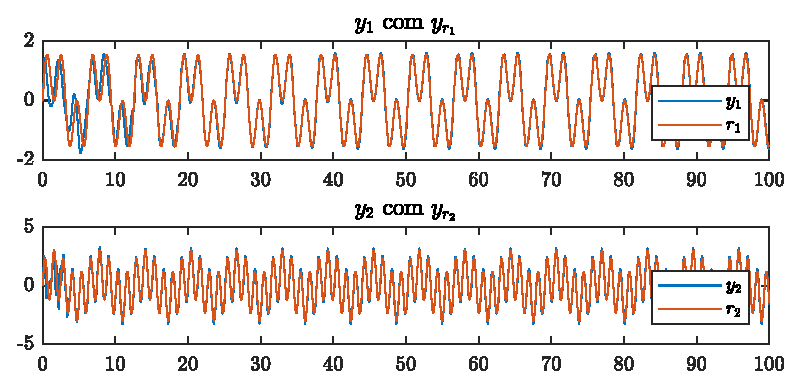
\includegraphics[width=12cm]{figs/y/sim0_yr1yr2.eps} 
\end{figure}